\documentclass{article}
\usepackage{graphicx} % Required for inserting images

\title{test}
\author{Christian Magelssen}
\date{February 2024}

\begin{document}

\maketitle

\section{Introduction}

The hallmark of expertise lies in the flawless execution of actions and the selection of optimal choices to achieve goals  \cite{wolpert_principles_2011, krakauer_motor_2019, mangalam_investigating_2023, du_relationship_2022, gallivan_decision-making_2018}. These choices (or cognitive strategies) are typically trained with instruction-based approaches, where a coach tells learners what to do (e.g., take a shorter line around the gate) followed by corrective feedback (e.g., you can shorten the line even more) \cite{williams_practice_2005, williams_effective_2023, hodges_role_1999}. This teaching strategy can be likened to what motor learning refers to as supervised learning, where the teaching signal for skill improvement represents the disparity between the desired skill outcome and the learner outcome \cite{jordan_forward_1992, wolpert_motor_2010, doya_complementary_2000}. Through practice this teaching signal can bring the learner close to execute what is assumed to be the correct choice, but does this teaching strategy truly foster creativity and intelligent strategic choices, such as helping learners discover innovative and vastly more effective solutions that surpass our imagination?

One drawback of the supervised learning strategy for training these decisions is that learners are simply told what to do based on what coaches believe to be a good strategy from their knowledge or experience. However, what coaches judge as a good strategy does not always align with reality, even for the best-trained eye \cite{supej_impact_2019, cochrum_visual_2021}. Learners might, therefore, miss opportunities to discover the best strategy when coaches opt for suboptimal choices. Supervised learning might also constrain learners to adopting a single ('universal') strategy for all situations rather than acquiring a repertoire of strategies and discerning the most effective strategies for each specific scenario. Finally, it remains uncertain whether the prescriptive approach is the most effective teaching strategy for achieving long-lasting learning effects \cite{wulf_instructions} 

Learning to make good choices can also happen without the direct influence of a coach who gives advice. The cornerstone of reinforcement learning \cite{sutton_reinforcement_2018} is that learners can learn by exploring strategies and evaluating their outcomes, using the successes and failures of outcomes as teaching signals. That is, rather than being told the putatively correct solution to the problem, as in supervised learning, they learn about the value of different strategies, which allows them to pick the best solution. These values are learned by comparing a given choice's outcomes with the currently expected outcome of that choice. Outcomes that exceed or fall short of expectations result in errors in reward prediction, signaling that the learner must update their predictions to better anticipate future rewards following that action \cite{rescorla_theory_1972}. These reward prediction errors are then incorporated to form a new and better estimate of reward, by updating expectations through a weighted running average. Reinforcement learning has been tremendously powerful in explaining human and animal learning \cite{waelti_dopamine_2001, schultz_neural_1997, pessiglione_dopamine-dependent_2006}, as well as training AI to perform complex tasks such as computer games starting from pixel inputs, only\cite{mnih_human-level_2015}. Given this evidence, could reinforcement learning offer an alternative to standard coach-based supervised learning to improve skill learning for skilled performers?

A critical knowledge gap in motor learning concerns how learners use explicit strategies to achieve goals and how these strategic decisions develop and improve over time. Previous studies have shown that motor skill learning through reinforcement learning can slow the learning process \cite{lior_shmuelof_overcoming_2012}, but enhance off-line gains, resulting in improved retention \cite{hasson_reinforcement_2015, therrien_effective_2016, lior_shmuelof_overcoming_2012, truong_error-based_2023}. Reinforcement learning is also presumed to exert great influence on strategic choices and learning, despite this being little explored. Therefore, we asked whether reinforcement learning improves strategy learning among high-performing learners compared to traditional supervised learning with a coach. 

To address this question, we conducted a three-day learning experiment with ninety-eight skilled and elite alpine ski racers from Norway and Sweden. To facilitate skill development in this skilled group of athletes, we selected a section of a slalom course where there is great improvement potential, even among the best skiers. This skill was to improve times on flat sections in slalom, and we defined four strategies intentionally to enhance this skill (\ref{fig:courseandstrategies}b). Our hypothesis was that skiers in the reinforcement learning group would learn to choose better strategies and thus achieve better performance than skiers subject to traditional supervised learning with a coach. To test this, we assigned skiers to three different learning groups with different instructions and feedback (Fig. \ref{fig:experiment}b): In the reinforcement learning group, skiers chose a strategy on every run and saw their race times to inform these decisions. In the supervised (free choice) learning group, a ski coach made this choice for the skier, while in the supervised (target skill) learning group, we recruited current World-Cup ski coaches to instruct skiers to select the strategy that we defined as the theoretically best strategy based on computational modeling \cite{lind_physics_2013} and observations of elite skiers \cite{reid_alpine_2020}. Coaches in the two supervised learning groups saw the times but were instructed not to disclose them to the skiers. 

We found that the reinforcement learning group showed greater improvement during acquisition and performed better in retention compared to the supervised (free choice) learning group. We observed an improvement in strategy choices for both reinforcement learning and supervised (free choice) learning groups, but we did not observe any statistically significant differences in choices between groups, either for the theoretically best strategy or individual skiers' estimated best strategy. We also found that both groups were sensitive to performance feedback, exhibiting win-stay, lose-shift behavior in strategy choices, but the descriptively greater sensitivity to feedback in the \textbf{}reinforcement learning group was not statistically significant. Our results suggest that reinforcement learning yields comparable outcomes to supervised learning, and that any advantages of reinforcement learning over supervised learning are more likely rooted in effects on skill execution rather than action selection. 



\begin{figure}[h!]
\centering
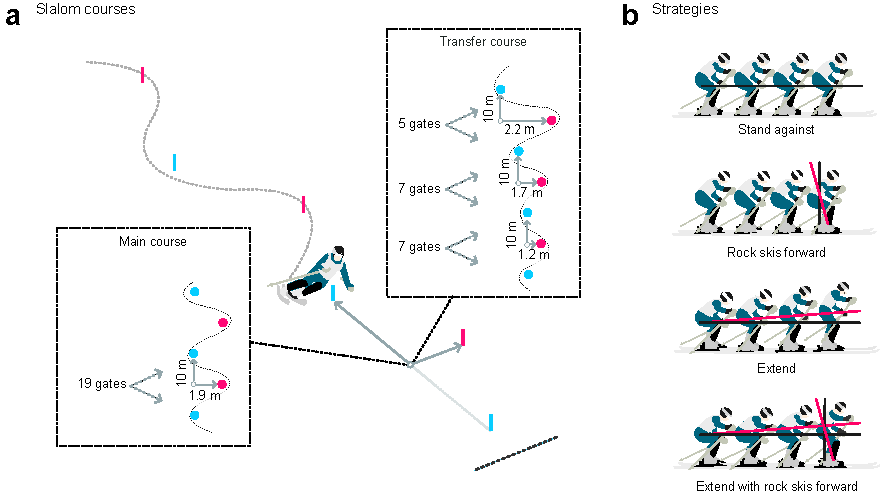
\includegraphics{figures/figure_method_courseandstrategy.pdf}
\caption{\textbf{a.} Illustrations of the two slalom courses used in the study. The main slalom course was a rhythmic course deployed in all sessions except for the transfer test. The course setting for the transfer test involved a progression in gate offset, starting with the largest offset and ending with the smallest offset. \textbf{b.} Illustration of the strategies defined to enhance racing performance on flat terrain in slalom: The "stand against" strategy emphasized maintaining a stable stance against external forces without body extension along the body's longitudinal axis or rocking skis forward; 'Rock skis forward' involved rocking skis forward from gate passage to completion of the turn; The "extend" strategy involves extending the body from a laterally tilted position during the turn, closer to the turn's center of rotation; The "extend with rocking skis forward" was expected to be the best strategy combining the two effects from extending and rocking skis forward, and we therefore defined this as the theoretical best strategy}
\label{fig:courseandstrategies}
\end{figure}

\begin{figure}[h!]
\centering
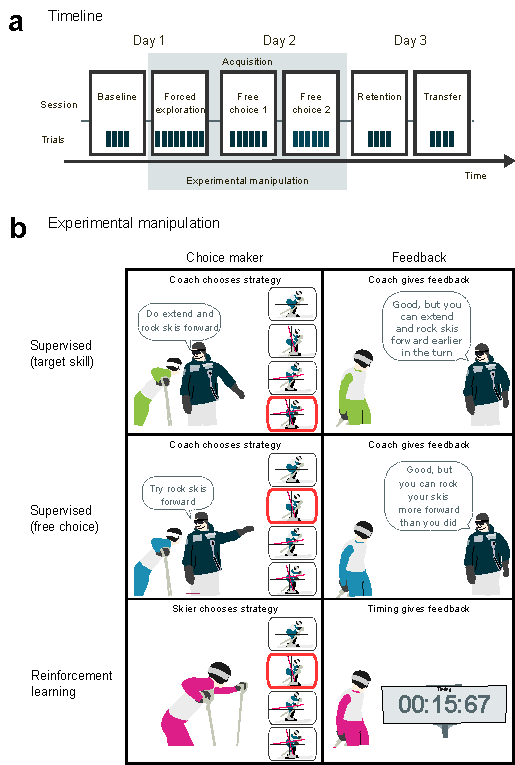
\includegraphics{figures/figure_method_experiment.pdf}
\caption{Illustration of the experimental design and procedure.Timeline of the three-day skill learning experiment. During the baseline, skiers skied a slalom course as fast as they could without receiving racing time feedback. The skiers' performances were ranked to form blocks. Within each block, skiers were randomly assigned to one of three treatment groups (see b).Skiers underwent an acquisition phase in their designated treatment group comprising one forced exploration and two free-choice sessions. On the last day, skiers completed a retention and transfer test, again without feedback from coaches nor timing. Illustration of treatment groups in the study. Supervised (target skill) involved coaches consistently choosing the theoretically best strategy, while supervised (free choice) allowed coaches to select strategies freely. Skiers in both these treatment groups received feedback on strategy execution from their respective coach, while skiers in the reinforcement learning group independently selected strategies and received feedback from the timing system to facilitate value learning of each strategy. }
\label{fig:experiment}
\end{figure}



\section{Discussion}

Expert performance hinges on the selection and precise execution of effective strategies. The standard approach to training these decisions is to inform learners what strategy to select. Our study suggests that reinforcement learning can complement this traditional training strategy and offer an alternative for developing decision expertise more purposefully.

We found that reinforcement learning improved race times more during the acquisition phase and performed better during retention than supervised (free-choice) learning. Both treatment groups chose better strategies during the sessions, with a clear 'win-stay, lose-switch' signature showing that they tended to stick to successful strategies. Despite the descriptively greater tendency for reinforcement learning to select better strategies and to have more pronounced "win-stay, lose-switch" tendencies during acquisition, these differences were not significantly different, nor were their contrasts at any of the sessions. However, we found that reinforcement learning had lower costs for suboptimally chosen strategies, indicating that the skiers had acquired a better cognitive understanding of the strategies' effect. However, this explanation does not comprehensively account for the disparity in race time. Compared with supervised (free choice) learning, reinforcement learning achieved greater improvement in the 'extend' strategy, suggesting that reinforcement feedback might have increased motor motivation. However, the reinforcement learning group did not outperform the supervised (target skill) learning group. This speaks to the importance of learning strategies. Interestingly, despite their clear difference in race time, the supervised (target skill) learning group did not significantly differ between the 'extend' and 'rock skis forward' strategies, suggesting the benefits of exposing learners to various strategies. Overall, we suggest that coaches can enhance skill learning by developing strategies and allowing learners to gain insights into their causal effects from evaluations instead of pure instruction.

A crucial and intriguing finding was that reinforcement learning outperformed supervised (free choice) learning in retention. The findings accords with earlier 'discovery' based approach that reported better learning in absence of instruction. This finding aligns with prior research showing that reinforcement learning enhances retention \cite{smuilof, 2002}. The presumed explanation behind these findings is that reinforcement enhances offline improvement of motor memories that is not observed with other learning paradigms. 

Our hypothesis, however, was that reinforcement learning learned to make better strategy choices than supervised (free choice) by learning from evaluations instead of instructions. We did not find corroborating evidence for this hypothesis, however. On retention, the

but we found that the costs of choosing suboptimal strategies on retention was significantly lower in reinforcement learning than in supervised (free choice) learning. 






One explanation for this is that the coaches in the supervised (free choice) learning were highly experienced and merited coaches, but who also learned extensively from the experiment. This is evident from seeing the strategies ranking approaching the observed race times. As such, they too learned extensively from the project and that may have prevented the the effect to play in full. 

An interesting observation was that the 




Vår hypotese var imidlertid at reinforcement learning forbedret prestasjonen fordi de valgte bedre strategier enn supervised (learning) gruppen. 


A surprising finding was that the predicted probability of choosing the estimated best strategy decreased from free choice 2 to retention for reinforcement learning. At the same time, it increased for the supervised (free choice) learning group, leading to a significant interaction effect. This difference in change resulted in supervised learning (free choice) actually having a marginally higher predicted probability of choosing the estimated best strategy, contrary to our hypothesis. Nevertheless, we found that reinforcement learning skied better in retention and incurred lower costs (measured as regret) from their supoptimal chosen strategies compared to supervised (free choice) learning. One interpretation of this result is that skiers also took into account the risk associated with the execution of strategies, opting for those with lower risk. In that case, one might consider that "extend with rock skis forward" could be more exposed to risk since it could potentially make athletes lean to far backward to make the next turn.  However, this does not seem to be the case, as observed from both Figure 5a and the raw data in Figure 4, where the choices of this strategy have increased. Therefore, it appears that, at least on average, this is not a good account of our data. A more likely one is that that the skiers in reinforcement learning better grasped the effects of the different strategies and learned that some strategies were equally effective so that it did not matter much which they chose.

Our data can also be explained in a neuroeconomic framework \cite{pietro_mazzoni_why_2007, dudman_basal_2016}  by reinforcement learning increasing motor vigor. Executing repetitive up-and-down movements down a slalom course using the 'extend' and 'extend with rock skis forward' strategies is more energy expensive than performing the 'stand against' or 'rock skis forward' strategies. Besides having the energy to choose these strategies, it is possible that reinforcement learning had higher motor vigor when performing these strategies. That is, they performed the strategies with more power and quicker execution, which generally translates into better performance in ski racing given the snow resists the forces without being compressed. Previous studies on vigor have found that people make saccades \cite{takikawa_modulation_2002} and reach\cite{summerside_vigor_2018} faster towards targets paired with rewards than unpaired targets. It is therefore possible that the reinforcement learning increased motor vigor. Comments from several coaches, who watched the retention and transfer, from the sideline, was that the skiers in the reinforcement learning group tended to use more arm movements than skiers in the other groups, despite the instruction did not tell them to do that. The vigor perspective may also help explaining why reinforcement learning did not learn better than the supervised (target skill) learning group, as previous studies also have found that training with explicit knowledge boosts motor vigor much like the effect of reward itself \cite{anderson_rewards_2020, wong_explicit_2015}. It may therefore be that the getting information that one strategy was best from a current World Cup coach may have boosted the implicit motivation to perform this strategy well. 






Det samsvarer også med eldre studier innenfor mer discovery learning som viser at læring under eksplisitt instruksjoner kan være gunstig for læring. Tidligere 




, suggesting that strategy selection may have played an important role in learning. Interestingly, the supervised (target skill) learning group struggled to differentiate between the 'extend' and 'rock skis forward' strategies despite their clear race time difference, suggesting the benefits of exposing learners to various strategies. Exposing learners to different strategies might therefore be beneficial. Taken collectively, we suggest that coaches can enhance skill learning by developing strategies within their sport and allowing athletes to evaluate them, rather than always instructing learners.

Retention...

Our hypothesis was that reinforcement learning improves transfer to a new slalom course. The rationale for such expected behaviour was that reinforcement learning would achieve better insights into to the strategies' effect, thereby promoting better decision-making in new situations. However, we found no corroborating evidence for this hypothesis. This result aligns with studies that have observed enhanced retention but not transfer with reinforcement compared to supervised learning \cite{hasson_reinforcement_2015}. Furthermore, reinforcement learning has been found to yield a lower generalization signature in adaptive tasks \cite{lior_shmuelof_overcoming_2012}. One account for these findings is that reinforcement learning improves learning only for the specific situations in which one has been rewarded, as these are the instances in which learning has been reinforced. A potential mechanism for this is that training with rewards shortens the time window during which memory is unstable, affecting learners' capacity to extend learning to new situations \cite{robertson_memory_2018}. It is also conceivable that a more structured learning approach, where learners are exposed to frequent switches between strategies, is necessary to grasp the task's structure and promote transfer \cite{braun_structure_2010}. Future research should possibly investigate the effect of structural learning. 





Our study suggests that reinforcement learning can be an essential training strategy to improve skill acquisition. However, before encouraging coaches and instructors to implement this strategy, we discuss the significance of the effect size and its amplifying and counteracting mechanisms for generalizability \cite{anvari_not_2023}. To start this discussion, we emphasize that the estimated effect size during retention was smaller than our predefined smallest effect size of interest. This benchmark, however, was set for a longer slalom course and more training sessions than we could execute due to space and time constraints in the ski hall. Consequently, we exercise caution in outright dismissing its practical significance. Instead, we aim to help the reader understand its potential importance for skill improvement in our sample of skiers. The first step towards this insight is to consider that the slalom course approximately equaled one-third of a full slalom race course, and a slalom race consists of two runs. Therefore, the 0.12 seconds effect size could be scaled up by a factor of 6, potentially proving significant for coaches in a more accurate course setup. However, racecourses consisting solely of flat sections are rare, and it is more realistic to assume that a flat section of a course constitutes only one-third of the entire course. If we base our understanding on this assumption, we can convert the 0.12-second difference into FIS world ranking positions. Considering that a race consists of two runs, this translates into an improved World Rank of 27 positions for females and 65 for males, based on a median ranking of 600 in our sample (see Supplement discussion). This could be of significant importance, but we have to remember that this effect cannot be directly transferred, as sports expertise also involves cognitive decisions \cite{mangalam_investigating_2023, krakauer_motor_2019}, such as switching from one strategy to another during a race. Our study did not capture such decisions as we focused on flat sections. In conclusion, the estimated effect could be larger if not because reinforcement learning and supervised learning conducted the retention and transfer tests simultaneously. This design choice allowed the skiers to observe each other, possibly diluting some of the effect. However, this decision was made to mirror the conditions of alpine competitions and gave us confidence that athletes experienced similar conditions during testing. 






\end{document}
